Dette appendix indeholder billeder og figure fra dokumentationen, som det ikke var hensigtsmæssige at medtage i det øvrige dokument.

\begin{figure}[h]
\centering
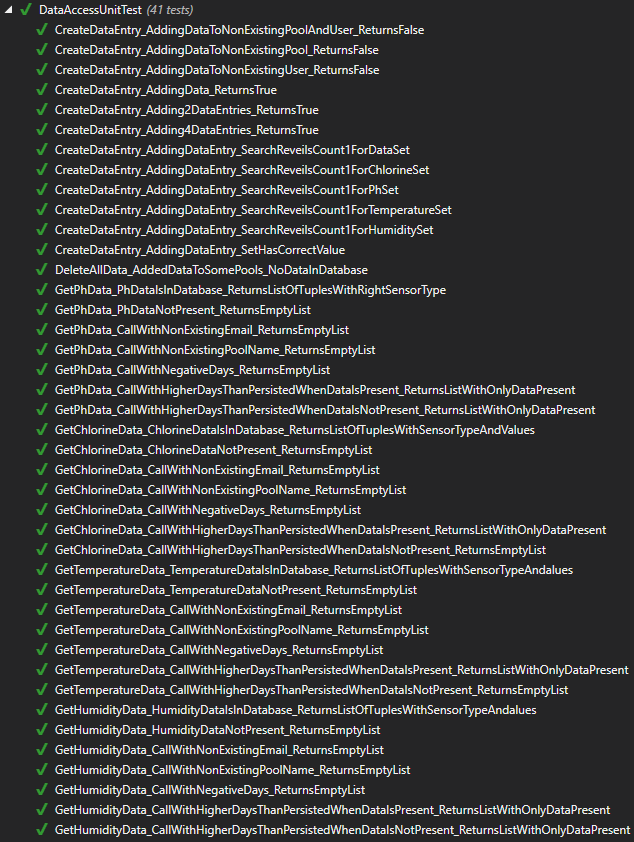
\includegraphics[width=0.7\linewidth]{figs/test/dataaccessunittest_appendix.png}
\caption{Unittest for DataAccess.}
\label{fig:dataaccessunittest_appendix}
\end{figure}

\begin{figure}[h]
\centering
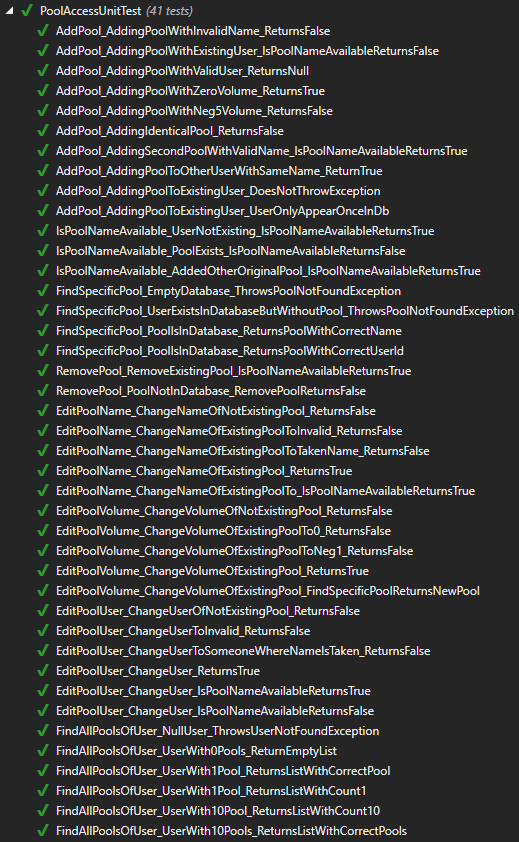
\includegraphics[width=0.7\linewidth]{figs/test/poolaccessunittest_appendix.png}
\caption{Unittest for PoolAccess.}
\label{fig:poolaccessunittest_appendix}
\end{figure}

\begin{figure}[h]
\centering
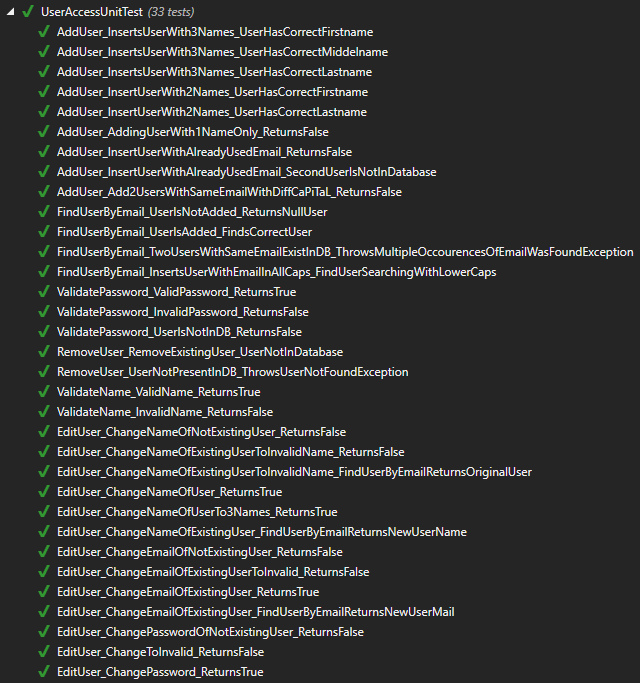
\includegraphics[width=0.8\linewidth]{figs/test/useraccessunittest_appendix.png}
\caption{Unittest for UserAccess.}
\label{fig:useraccessunittest_appendix}
\end{figure}

\begin{landscape}
	\begin{figure}[h]
		\centering
		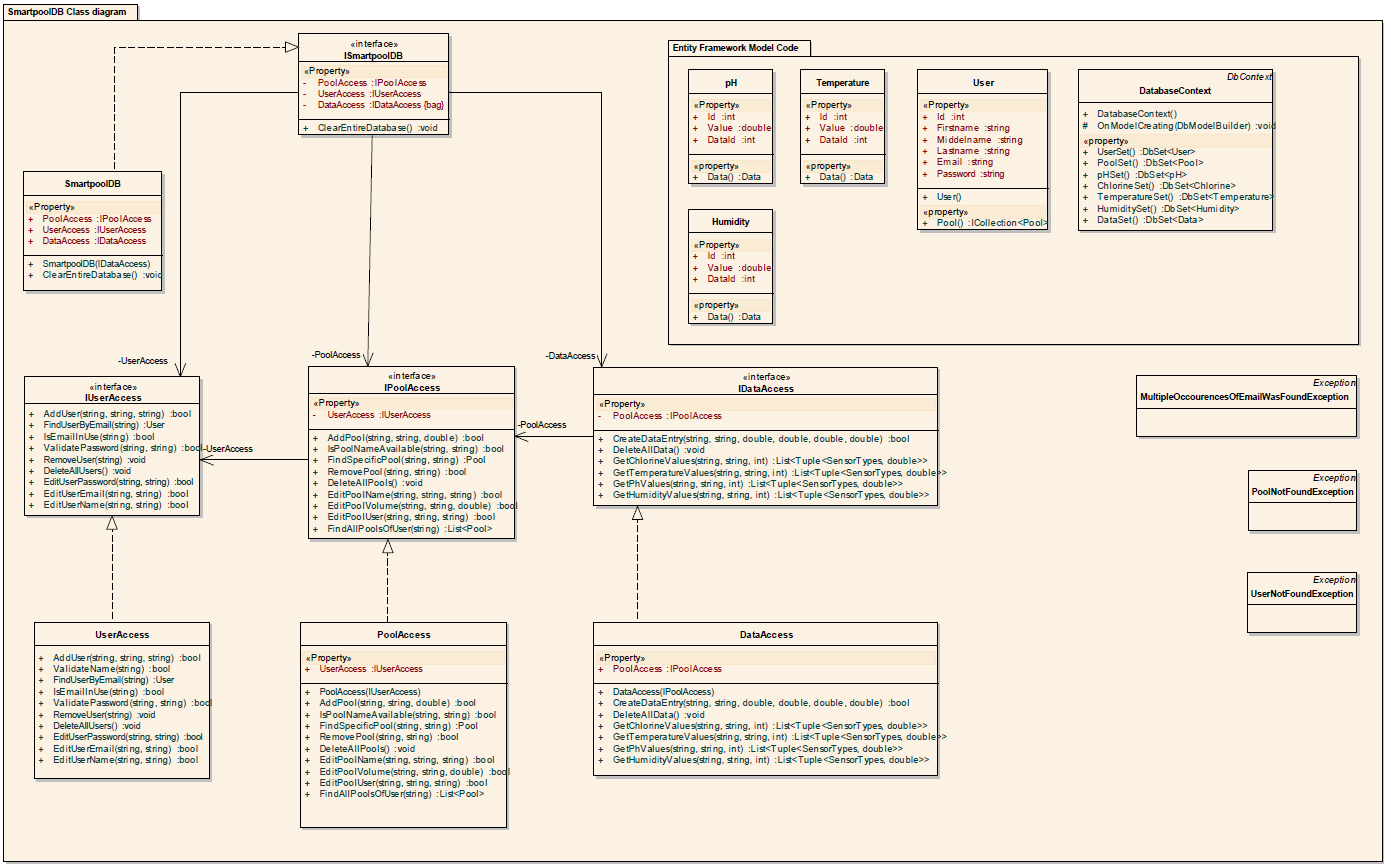
\includegraphics[width=\linewidth]{figs/implementering/databaseFullClass.PNG}
		\caption{Database access klassediagram}
		\label{fig:databaseFullClass}
	\end{figure}
\end{landscape}

\begin{figure}
\centering
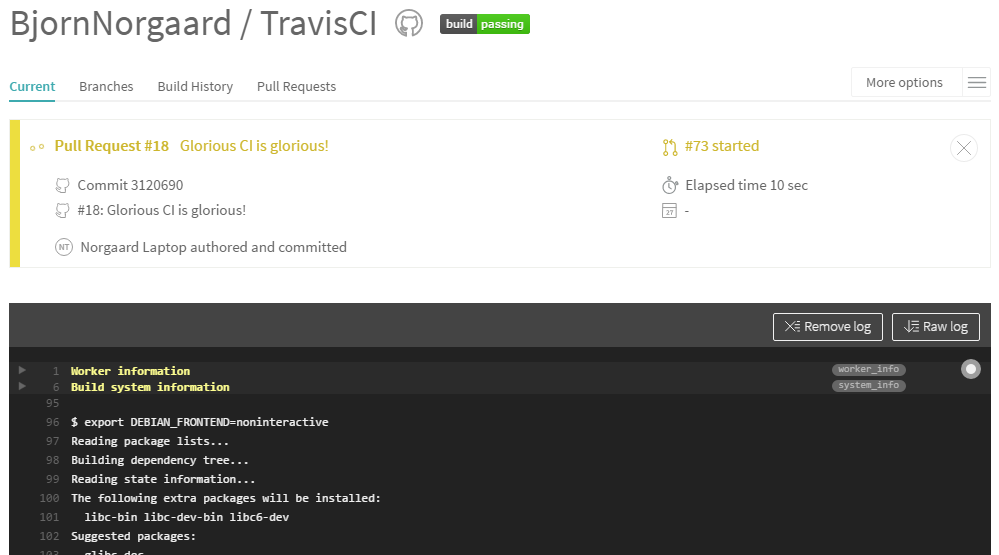
\includegraphics[width=\linewidth]{figs/travis/travisbuildstarted}
\caption{Travis CI, web interface hvor et byg er begyndt.}
\label{fig:travisbuildstarted}
\end{figure}

\begin{figure}
\centering
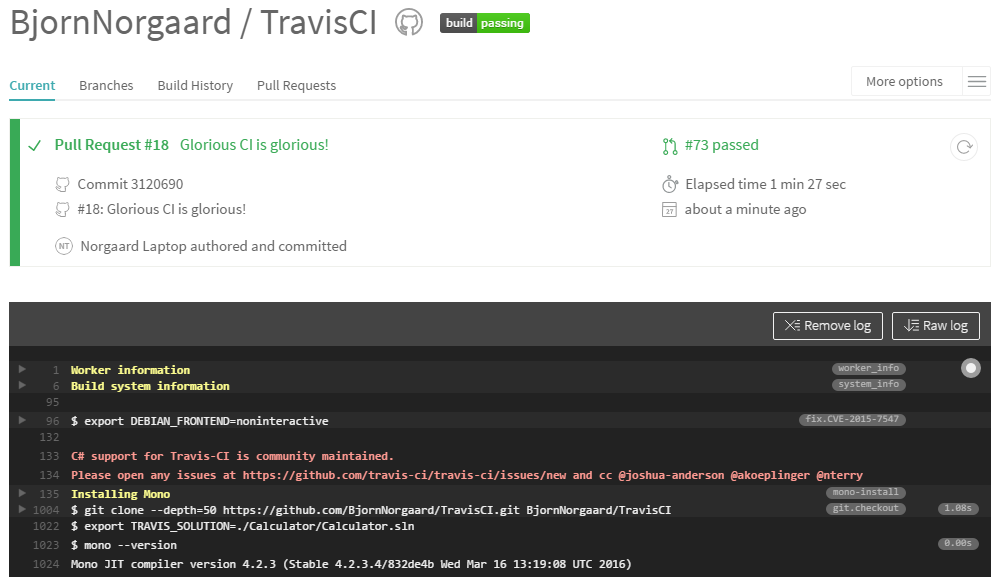
\includegraphics[width=0.7\linewidth]{figs/travis/travisbuildsuccess}
\caption{Travis CI, web interface hvor et byg er lykkeds.}
\label{fig:travisbuildsuccess}
\end{figure}

\begin{figure}
\centering
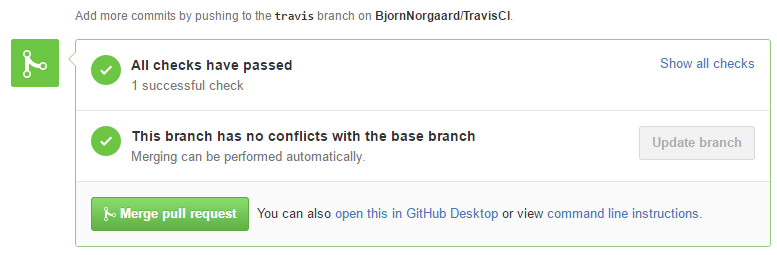
\includegraphics[width=0.7\linewidth]{figs/travis/travisgithubsuccess}
\caption{Travis CI, github interface hvor et byg er lykkeds.}
\label{fig:travisgithubsuccess}
\end{figure}

\begin{figure}
\centering
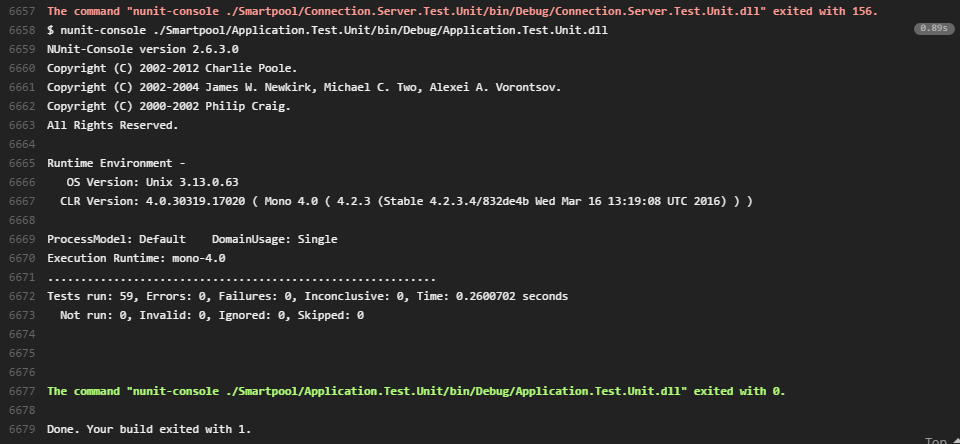
\includegraphics[width=0.7\linewidth]{figs/travis/travisoutput}
\caption{Travis CI, output efter succesfuldt byg.}
\label{fig:travisoutput}
\end{figure}

\begin{figure}
\centering
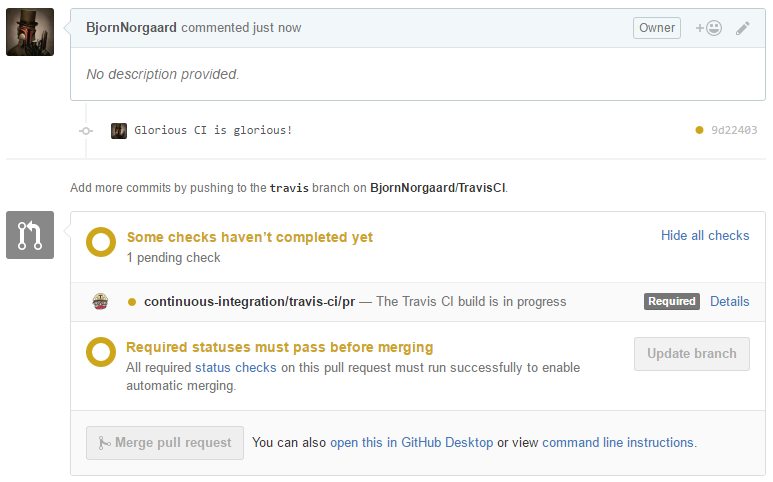
\includegraphics[width=0.7\linewidth]{figs/travis/travispullrequest}
\caption{Travis CI, github efter byg er started}
\label{fig:travispullrequest}
\end{figure}

\begin{figure}
\centering
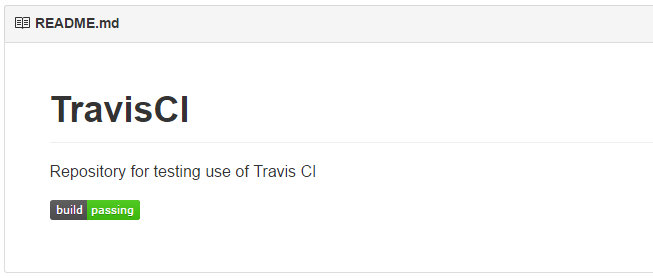
\includegraphics[width=0.7\linewidth]{figs/travis/travisreadme}
\caption{github readme, med travis status}
\label{fig:travisreadme}
\end{figure}

\begin{figure}
\centering
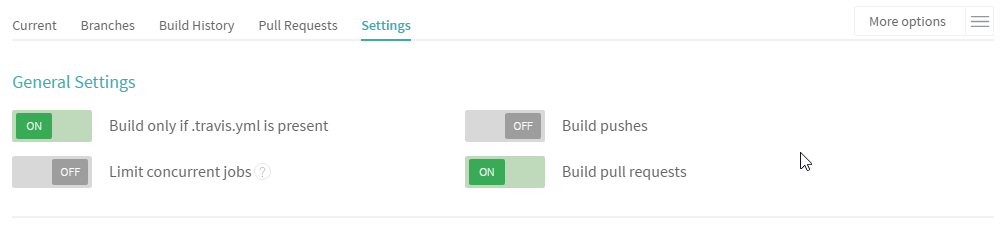
\includegraphics[width=0.7\linewidth]{figs/travis/travissettings}
\caption{Travis CI, indstillinger for repo.}
\label{fig:travissettings}
\end{figure}
